\documentclass[11pt]{article}
\usepackage{mathblatt}
\usepackage{eigene}
\usepackage[hidelinks]{hyperref}
\newcommand{\vz}[2]{\noindent\hyperlink{#1}{#2}\par\smallskip}
\begin{document}
\blattkopf{Daten}{Lernblatt}
\eng
\noindent\textbf{\large Inhalt}\par\medskip
\vz{b0}{Blatt 0 · Das kannst du schon (Nr. 1--7) · Seiten 2--3}
\vz{e1}{Einheit 1 · Häufigkeiten (Nr. 8--13) · Seiten 4--6}
\vz{e2}{Einheit 2 · Säulen-, Balken- und Liniendiagramme (Nr. 14--21) · Seiten 7--12}
\vz{e3}{Einheit 3 · Streifen- und Kreisdiagramm (Nr. 22--28) · Seiten 13--15}
\vz{e4}{Einheit 4 · Kenngrößen (Nr. 29--35) · Seiten 16--18}
\vz{e5}{Einheit 5 · Diagramme beurteilen und Boxplot (Nr. 36--40) · Seiten 19--21}
\weit
\clearpage\hypertarget{b0}{}\noindent\textbf{Blatt 0 · Das kannst du schon}
\setcounter{aufgabe}{0}

\begin{aufgabe}{Prozente -- rechnen und umrechnen. Rechne, wo es geht, im Kopf.}
\begin{teile}
\teil 30 von 100 Stiften sind rot. \feld[\%]{p}
\teil 7 von 100 Feldern sind grau. \feld[\%]{p}
\teil Schreibe als Prozent: $0{,}45$ \leerfeld[\%]
\teil Schreibe als Dezimalzahl: $8\,\%$ \leerfeld
\teil 12 von 48 Kindern haben ein Instrument gelernt. \feld[\%]{p}
\teil In einer Klasse fahren $45\,\%$ mit dem Rad und $30\,\%$ mit dem Bus, der Rest geht zu Fuß. \feld[\%]{p}
\end{teile}
\end{aufgabe}

\begin{aufgabe}{Zahlen ordnen und Skalen ablesen.}
Ordne von klein nach groß.
\begin{teile}
\teil $4{,}7 \quad 4{,}07 \quad 4{,}71 \quad 4{,}17$ \\[2pt] \leerfeld\ $<$ \leerfeld\ $<$ \leerfeld\ $<$ \leerfeld
\teil $12{,}5 \quad 9{,}8 \quad 12{,}05 \quad 9{,}75$ \\[2pt] \leerfeld\ $<$ \leerfeld\ $<$ \leerfeld\ $<$ \leerfeld
\end{teile}

Lies die Zahlen am Zahlenstrahl ab.

\zahlenstrahl[xmin=0,xmax=5,xstep=0.5,karo=1.4]{1.5/A, 3.25/B, 4.75/C}

\begin{teilezwei}
\tz $A =$ \leerfeld & \tz $B =$ \leerfeld \\
\tz $C =$ \leerfeld & \\
\end{teilezwei}
\begin{teile}
\teil Auf einer Achse sind die Linien mit $0$, $50$, $100$, $150$ beschriftet. Zwischen zwei beschrifteten Linien liegen vier dünne Hilfslinien. Wie viel ist ein Schritt von Linie zu Linie wert? \leerfeld
\end{teile}
\end{aufgabe}

\begin{aufgabe}{Winkel und Anteile am Vollkreis.}
\begin{teile}
\teil Ein Vollkreis hat \leerfeld[$^\circ$]
\teil Ein Viertel des Vollkreises: \leerfeld[$^\circ$]
\teil Die Hälfte des Vollkreises: \leerfeld[$^\circ$]
\teil Ein Drittel des Vollkreises: \leerfeld[$^\circ$]
\teil Ein Zehntel des Vollkreises: \leerfeld[$^\circ$]
\teil Ein Winkel misst $45^\circ$. Welcher Anteil des Vollkreises ist das? \leerfeld
\teil Trage am Strahl mit dem Geodreieck einen Winkel von $70^\circ$ an.
\end{teile}

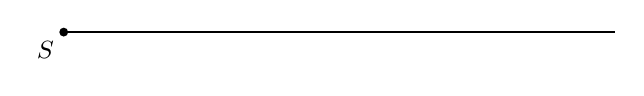
\begin{tikzpicture}
  \draw[line width=0.7pt] (0,0) -- (7,0);
  \fill (0,0) circle (1.6pt) node[below left,font=\small] {$S$};
\end{tikzpicture}
\end{aufgabe}

\begin{aufgabe}{Zentimeter und Millimeter.}
\begin{teilezwei}
\tz $3\,$cm $=$ \leerfeld[mm] & \tz $45\,$mm $=$ \leerfeld[cm] \\
\tz $7{,}2\,$cm $=$ \leerfeld[mm] & \tz $10\,$cm $=$ \leerfeld[mm] \\
\end{teilezwei}
\begin{teile}
\teil Trage auf der Linie vom linken Ende aus $6{,}5\,$cm ab und markiere die Stelle mit einem Strich.
\end{teile}

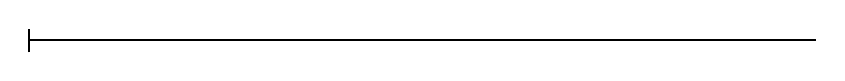
\begin{tikzpicture}
  \draw[line width=0.7pt] (0,0) -- (10,0);
  \draw[line width=0.7pt] (0,-0.15) -- (0,0.15);
\end{tikzpicture}
\end{aufgabe}

\begin{aufgabe}{Mit Dezimalzahlen rechnen und runden. Bei e) bis g) darfst du den Taschenrechner benutzen.}
\begin{teilezwei}
\tz $2{,}5 + 3{,}5 =$ \leerfeld & \tz $12 : 4 =$ \leerfeld \\
\tz $18{,}6 + 4{,}9 + 0{,}5 =$ \leerfeld & \tz $78 : 5 =$ \leerfeld \\
\tz $61{,}5 : 4 =$ \leerfeld & \\
\end{teilezwei}
\begin{teile}
\teil Runde dein Ergebnis aus e) auf eine Stelle nach dem Komma. \leerfeld
\teil Runde $3847{,}6$ auf Hunderter. \leerfeld
\end{teile}
\end{aufgabe}

\begin{aufgabe}{Bruchteil und Vielfaches einer Zahl.}
\begin{teilezwei}
\tz Die Hälfte von $60$: \leerfeld & \tz Ein Drittel von $90$: \leerfeld \\
\tz Ein Viertel von $70$: \leerfeld & \tz Doppelt so viel wie $45$: \leerfeld \\
\end{teilezwei}
\begin{teile}
\teil Ein Drittel mehr als $210$ -- wie viel ist das? \leerfeld
\teil Von den Befragten nennt jede fünfundzwanzigste Person Tennis. Wie viel Prozent sind das? \leerfeld[\%]
\end{teile}
\end{aufgabe}

\begin{aufgabe}{Fehler finden -- Anteile in Prozent.}
In einer Gruppe von 36 Jugendlichen haben 27 ein eigenes Fahrrad. Tim will wissen, wie viel Prozent das sind, und rechnet:
\rechnung{27 : 9 &= 3 \\ &= 300\,\%}
\begin{teile}
\teil Finde den Fehler, benenne ihn und schreibe die richtige Rechnung auf. \\[10pt]
\teil Von 60 Besuchern kaufen 21 ein Getränk. Wie viel Prozent sind das? \feld[\%]{p}
\end{teile}
\end{aufgabe}

\clearpage\hypertarget{e1}{}\setcounter{aufgabe}{7}
\einheitenkopf{Einheit 1 von 5 · Häufigkeiten}

\begin{aufgabe}{Häufigkeiten -- Was ist das Ganze? Unterstreiche im Text die Zahl, die das Ganze angibt, und schreibe sie ins Feld. Rechne noch nicht.}
\begin{teile}
\teil In einer Woche fanden 18 Spiele statt. 7 davon gewann die Mannschaft. \leerfeld
\teil Von den 250 Besuchern kamen 90 mit dem Fahrrad. \leerfeld
\teil In einer Klasse sind 14 Mädchen und 12 Jungen. 9 von ihnen spielen ein Instrument. \leerfeld
\teil An der Umfrage nahmen 40 Personen teil. 6 nannten Tennis, 14 Fußball, die übrigen Handball. \leerfeld
\teil In einer Kiste liegen 12 rote, 8 blaue und 5 grüne Kugeln. Welchen Anteil haben die blauen? \leerfeld
\end{teile}
\end{aufgabe}

\begin{aufgabe}{Häufigkeiten -- auszählen. Zähle die Striche aus und schreibe die Anzahl in die rechte Spalte.}
\beispiel{\text{\strichliste{|||||\ ||}} \quad &\rightarrow\quad 7}

\sachtabelle{lcc}{Farbe & Strichliste & Anzahl}{%
a) Rot & \strichliste{|||||\ |||} & \leerzelle \\
b) Blau & \strichliste{|||||\ |||||\ ||} & \leerzelle \\
c) Grün & \strichliste{||||} & \leerzelle \\
d) Gelb & \strichliste{|||||\ |||||\ |||||\ |} & \leerzelle}

\begin{teile}
\setcounter{teil}{4}
\teil Beim Würfeln wurden diese Augenzahlen notiert (Urliste):
\par\smallskip
\noindent 3\; 5\; 1\; 3\; 6\; 3\; 2\; 5\; 3\; 1\; 6\; 4\; 3\; 2\; 5\; 3\; 6\; 1\; 4\; 3
\par\smallskip
Trage die Anzahlen in die Häufigkeitstabelle ein.
\end{teile}

\sachtabelle{lcccccc}{Augenzahl & 1 & 2 & 3 & 4 & 5 & 6}{%
Anzahl & \leerzelle & \leerzelle & \leerzelle & \leerzelle & \leerzelle & \leerzelle}
\end{aufgabe}

\begin{aufgabe}{Häufigkeiten -- rechnen. Gib bei a) bis e) die relative Häufigkeit als Bruch an.}
\beispiel{\text{9 von 12:}\quad h &= \tfrac{9}{12}}
\begin{teilezwei}
\tz 3 von 10 \leerfeld & \tz 7 von 20 \leerfeld \\
\tz 9 von 25 \leerfeld & \tz 4 von 50 \leerfeld \\
\end{teilezwei}
\begin{teile}
\teil 6 von 24 -- kürze den Bruch so weit wie möglich. \leerfeld
\end{teile}

Jetzt als Dezimalzahl oder in Prozent. Du darfst den Taschenrechner benutzen.
\begin{teile}
\teil 13 von 20 -- als Dezimalzahl. \feld{h}
\teil 17 von 40 -- als Dezimalzahl und in Prozent. \feld{h} \leerfeld[\%]
\teil 5 von 9 -- in Prozent, gerundet auf eine Stelle nach dem Komma. \leerfeld[\%]
\teil In einer Umfrage antworten $45\,\%$ „ja“ und $35\,\%$ „vielleicht“, die übrigen „nein“. Prüfe, ob die drei Anteile zusammen $100\,\%$ ergeben, und gib den fehlenden Anteil an. \leerfeld[\%]
\teil Lies im Diagramm ab, wie viele Jugendliche Tanzen nennen und wie viele insgesamt befragt wurden. Gib die relative Häufigkeit für Tanzen in Prozent an. \leerfeld[\%]
\end{teile}

\noindent\saeulen{Fußball/12,Tanzen/9,Rad/15,Judo/4}{18}{3}{Anzahl}

\begin{teile}
\teil Ein Verein hat 320 Mitglieder. $15\,\%$ von ihnen sind jünger als 12 Jahre. Wie viele Mitglieder sind das? \leerfeld
\teil Eine Mannschaft bestritt in einer Saison 40 Spiele. Sie gewann 26 Spiele, die übrigen verlor sie. Gib die relative Häufigkeit der Siege als Bruch und in Prozent an. (P10 2015)
\par \feld{h} \leerfeld[\%]
\end{teile}
\end{aufgabe}

\begin{aufgabe}{Häufigkeiten -- Fehler finden.}
In einer Klasse mit 32 Kindern haben 8 einen Hund. Mia gibt als relative Häufigkeit an:
\rechnung{h &= 8}
\begin{teile}
\teil Finde den Fehler, benenne ihn und schreibe die richtige Rechnung auf. \\[12pt]
\teil In einer Gruppe von 45 Personen tragen 18 eine Brille. Gib die relative Häufigkeit als gekürzten Bruch und in Prozent an. \par \feld{h} \leerfeld[\%]
\end{teile}
\end{aufgabe}

\begin{aufgabe}{Häufigkeiten -- Begründen. Rechne bei b) nicht mit dem Taschenrechner.}
\begin{teile}
\teil Erkläre, warum man zwei verschieden große Gruppen nur mit relativen Häufigkeiten vergleichen kann und nicht mit den Anzahlen. \\[12pt]
\teil In der 7a haben 12 von 24 Kindern ein Haustier, in der 7b sind es 15 von 30. In welcher Klasse ist der Anteil größer? Begründe. \\[12pt]
\end{teile}
\end{aufgabe}

\begin{aufgabe}{Häufigkeiten -- Anwendung. An zwei Schulen wurde gezählt, wie viele Kinder mit dem Rad kommen: an der Nordschule 84 von 240 Kindern, an der Südschule 78 von 195 Kindern.}
\begin{teile}
\teil Gib für beide Schulen die relative Häufigkeit in Prozent an.
\par Nordschule \leerfeld[\%] \quad Südschule \leerfeld[\%]
\teil An welcher Schule kommen mehr Kinder mit dem Rad? \leerfeld
\teil An welcher Schule ist der Anteil der Radfahrenden größer? \leerfeld
\teil Die Stadt baut zuerst an der Schule mit dem größeren Anteil neue Fahrradständer. Welche Schule ist das, und warum reicht die Anzahl aus b) für diese Entscheidung nicht aus? \\[12pt]
\end{teile}
\end{aufgabe}

\clearpage\hypertarget{e2}{}\setcounter{aufgabe}{13}
\einheitenkopf{Einheit 2 von 5 · Säulen-, Balken- und Liniendiagramme}

\begin{aufgabe}{Diagramm -- Was ist ein Kästchen wert? Gib nur an, wie viel ein Schritt von einer Linie zur nächsten wert ist. Lies keinen Wert ab.}
\begin{teile}
\teil Die Linien sind mit $0$, $10$, $20$, $30$ beschriftet, dazwischen liegt keine weitere Linie. \leerfeld
\teil Die Linien sind mit $0$, $100$, $200$ beschriftet, dazwischen liegt je eine Hilfslinie. \leerfeld
\teil Die Linien sind mit $0$, $20$, $40$, $60$ beschriftet, dazwischen liegen je drei Hilfslinien. \leerfeld
\teil Die Linien sind mit $0$; $0{,}05$; $0{,}10$ beschriftet, dazwischen liegen je vier Hilfslinien. \leerfeld
\teil Die Linien sind mit $0$, $200$, $400$ (in Mio.) beschriftet, dazwischen liegen je drei Hilfslinien. \leerfeld
\end{teile}
\end{aufgabe}

\begin{aufgabe}{Diagramm -- Wo fängt die Achse an? Kreuze an, ob die senkrechte Achse bei null beginnt. Wenn nicht, schreibe den Startwert auf.}
\begin{teile}
\teil Beschriftung $0$, $5$, $10$, $15$ \hfill \janein \quad Start: \leerfeld
\teil Beschriftung $40$, $45$, $50$, $55$ \hfill \janein \quad Start: \leerfeld
\teil Beschriftung $0$, $250$, $500$ \hfill \janein \quad Start: \leerfeld
\teil Beschriftung $3{,}10$; $3{,}15$; $3{,}20$ \hfill \janein \quad Start: \leerfeld
\teil Beschriftung $820$, $830$, $840$ \hfill \janein \quad Start: \leerfeld
\end{teile}
\end{aufgabe}

\begin{aufgabe}{Säulendiagramm -- ablesen. Das Diagramm zeigt, wie viele Gäste eine Eisdiele an den Tagen einer Woche hatte.}
\noindent\saeulenab[ymax=100,ystep=20,yfein=5,ylabel=Gäste]{Mo/20,Di/60,Mi/40,Do/80,Fr/55,Sa/75,So/65}

\begin{teilezwei}
\tz Montag \leerfeld & \tz Dienstag \leerfeld \\
\tz Mittwoch \leerfeld & \tz Donnerstag \leerfeld \\
\tz Freitag \leerfeld & \tz Sonntag \leerfeld \\
\end{teilezwei}
\begin{teile}
\teil An wie vielen Tagen kamen \emph{mehr als} 60 Gäste? \leerfeld
\teil An welchem Tag kamen die meisten, an welchem die wenigsten Gäste?
\par meiste: \leerfeld \quad wenigste: \leerfeld
\teil Wie viele Gäste kamen am Samstag mehr als am Mittwoch? \leerfeld
\end{teile}

Das zweite Diagramm zeigt die Zuschauerzahlen eines Stadions. Achte auf die Beschriftung der Achse.

\noindent\saeulenab[ymax=50,ystep=10,yfein=2,ylabel=Zuschauer in Tausend,breite=1.6]{2021/30,2022/24,2023/38,2024/46}

\begin{teile}
\teil Wie viele Zuschauer kamen 2022? \leerfeld
\teil Wie viele Zuschauer kamen 2024? \leerfeld
\teil Wie viele Zuschauer kamen 2024 mehr als 2021? \leerfeld
\end{teile}
\end{aufgabe}

\begin{aufgabe}{Balken- und Liniendiagramm -- ablesen. Das Balkendiagramm zeigt, wie oft vier Farben als Lieblingsfarbe genannt wurden.}
\noindent\balkenab[xmax=40,xstep=10,xfein=2,xlabel=Nennungen]{Rot/24,Blau/32,Grün/14,Gelb/8}

\begin{teilezwei}
\tz Rot \leerfeld & \tz Grün \leerfeld \\
\end{teilezwei}
\begin{teile}
\teil Welche Farbe wurde am häufigsten genannt? \leerfeld
\end{teile}

Das Liniendiagramm zeigt die mittlere Temperatur der ersten sechs Monate eines Jahres.

\noindent\liniendia[ymax=20,ystep=5,yfein=1,ylabel=Temperatur in $^\circ$C,breite=1.4]{Jan/2,Feb/5,Mär/4,Apr/9,Mai/14,Jun/17}

\begin{teile}
\teil Wie warm war es im März? \leerfeld
\teil In welchem Monat war es am kältesten? \leerfeld
\teil Zwischen welchen beiden Monaten ging die Temperatur zurück? \leerfeld
\teil Beschreibe in einem Satz, wie sich die Temperatur von März bis Juni verändert. \\[10pt]
\end{teile}
\end{aufgabe}

\begin{aufgabe}{Diagramm -- zeichnen. Ein Sportverein hat gezählt, wie viele Kinder die einzelnen Sportarten wählen.}
\sachtabelle{lccccc}{Sportart & Handball & Tennis & Judo & Reiten & Schwimmen}{%
Anzahl & 15 & 25 & 10 & 30 & 20}

Zeichne die Säulen in das vorbereitete Diagramm.

\noindent\saeulenab[ymax=40,ystep=10,yfein=5,ylabel=Anzahl,breite=1.7]{Handball/,Tennis/,Judo/,Reiten/,Schwimmen/}

\begin{teilezwei}
\tz Handball & \tz Tennis \\
\tz Judo & \tz Reiten \\
\end{teilezwei}
\begin{teile}
\teil Schwimmen
\teil Eine sechste Sportart wird von 75 Kindern gewählt. Was müsstest du an der senkrechten Achse ändern, damit auch diese Säule ins Diagramm passt? \\[10pt]
\end{teile}
\end{aufgabe}

\begin{aufgabe}{Diagramm -- Achseneinteilung. An der senkrechten Achse fehlen die Zahlen. Bekannt ist: Am Montag kamen 120 Besucher.}
\noindent\saeulenab[ymax=240,ystep=30,yfein=30,ylabel=Besucher,ohnezahlen,breite=1.6]{Mo/120,Di/180,Mi/90,Do/}

\begin{teile}
\teil Wie viele Besucher zeigt ein Kästchen? \leerfeld
\teil Wie viele Besucher kamen am Dienstag? \leerfeld
\teil Wie viele Besucher kamen am Mittwoch? \leerfeld
\teil Am Donnerstag kamen 210 Besucher. Zeichne die Säule ein.
\teil Das Diagramm unten zeigt für vier Sprachen, wie viele Menschen sie als Muttersprache sprechen. Beschriftet ist nur die Säule für Spanisch: 480 Mio. Außerdem ist bekannt: Hindi sprechen 320 Mio., Portugiesisch 240 Mio. und Arabisch 400 Mio. Menschen. Bestimme, wie viele Mio. ein Kästchen zeigt, schreibe „Hindi“ und „Portugiesisch“ anstelle der beiden Fragezeichen und zeichne die Säule für Arabisch ein. (P10 2023)
\end{teile}

\noindent\saeulenab[ymax=560,ystep=80,yfein=80,ylabel=Mio. Menschen,ohnezahlen,breite=1.8]{Spanisch/480,?/320,?/240,Arabisch/}
\end{aufgabe}

\begin{aufgabe}{Diagramm -- Fehler finden.}
An der senkrechten Achse eines Diagramms steht „Zuschauer in Tausend“. Die Säule für Samstag reicht genau bis zur Linie 18. Jonas notiert:
\rechnung{\text{Am Samstag kamen 18 Zuschauer.}}
\begin{teile}
\teil Finde den Fehler, benenne ihn und gib die richtige Zahl an. \\[10pt]
\teil Die Säule für Sonntag reicht auf derselben Achse bis 25. Wie viele Zuschauer kamen am Sonntag? \leerfeld
\end{teile}
\end{aufgabe}

\begin{aufgabe}{Diagramm -- Begründen.}
\begin{teile}
\teil Die Zahl der Geburten in einer Stadt soll für die Jahre 2015 bis 2024 dargestellt werden. Begründe, warum sich dafür ein Säulen- oder Liniendiagramm besser eignet als ein Kreisdiagramm. \\[12pt]
\teil Zwischen den beschrifteten Linien $0$ und $50$ liegen vier Hilfslinien. Jemand sagt: „Dann ist eine Hilfslinie 5 wert.“ Entscheide ohne Rechnung, ob das stimmen kann, und begründe. \\[12pt]
\end{teile}
\end{aufgabe}

\clearpage\hypertarget{e3}{}\setcounter{aufgabe}{21}
\einheitenkopf{Einheit 3 von 5 · Streifen- und Kreisdiagramm}

\begin{aufgabe}{Anteile -- Prozent oder Grad? Kreuze an, welche Einheit in die Lücke gehört. Rechne nicht.}
\begin{teile}
\teil Ein Viertel des Kreises ist ein Sektor von 90 \underline{\hspace{1cm}} \hfill \kreuz{\%}\kreuz{$^\circ$}
\teil Ein Viertel aller Befragten sind 25 \underline{\hspace{1cm}} \hfill \kreuz{\%}\kreuz{$^\circ$}
\teil Der ganze Kreis misst 360 \underline{\hspace{1cm}} \hfill \kreuz{\%}\kreuz{$^\circ$}
\teil Alle Anteile eines Kreisdiagramms ergeben zusammen 100 \underline{\hspace{1cm}} \hfill \kreuz{\%}\kreuz{$^\circ$}
\teil Von 200 Personen nennen 40 den Bus; ihr Sektor misst 72 \underline{\hspace{1cm}} \hfill \kreuz{\%}\kreuz{$^\circ$}
\end{teile}
\end{aufgabe}

\begin{aufgabe}{Anteile -- am Streifen. Der ganze Streifen ist 10\,cm lang und steht für $100\,\%$. Wie lang ist der Abschnitt?}
\beispiel{30\,\% \quad &\rightarrow \quad 3\,\text{cm}}
\begin{teilezwei}
\tz $40\,\%$ \leerfeld[cm] & \tz $20\,\%$ \leerfeld[cm] \\
\tz $70\,\%$ \leerfeld[cm] & \tz $5\,\%$ \leerfeld[cm] \\
\tz $45\,\%$ \leerfeld[cm] & \\
\end{teilezwei}
\begin{teile}
\teil Trage im Streifen die vier Abschnitte ab und beschrifte sie: Rad $25\,\%$, Bus $40\,\%$, zu Fuß $20\,\%$, Auto $15\,\%$.
\end{teile}

\noindent\streifenleer

\begin{teile}
\teil In einem anderen Streifen sind bereits $30\,\%$, $25\,\%$ und $20\,\%$ eingetragen. Wie viel Prozent fehlen noch? \leerfeld[\%]
\end{teile}
\end{aufgabe}

\begin{aufgabe}{Anteile -- Winkel berechnen. Berechne den Mittelpunktswinkel des Sektors.}
\beispiel{30\,\% \quad &\rightarrow \quad 0{,}30 \cdot 360^\circ = 108^\circ}
\begin{teilezwei}
\tz $50\,\%$ \leerfeld[$^\circ$] & \tz $25\,\%$ \leerfeld[$^\circ$] \\
\tz $10\,\%$ \leerfeld[$^\circ$] & \tz $75\,\%$ \leerfeld[$^\circ$] \\
\end{teilezwei}
\begin{teile}
\teil $12\,\%$ \leerfeld[$^\circ$]
\teil $37{,}5\,\%$ \leerfeld[$^\circ$]
\teil 8 von 25 Personen \leerfeld[$^\circ$]
\teil 15 von 400 Personen \leerfeld[$^\circ$]
\teil 3 von 7 Personen, gerundet auf eine Stelle nach dem Komma \leerfeld[$^\circ$]
\end{teile}
\end{aufgabe}

\begin{aufgabe}{Anteile -- Kreisdiagramm zeichnen. Nutze für a) bis c) den Kreis mit dem eingezeichneten Radius.}
\begin{teile}
\teil Trage vom Radius aus mit dem Geodreieck einen Sektor von $90^\circ$ an.
\teil Trage daran anschließend einen Sektor von $120^\circ$ an.
\teil Wie groß ist der Winkel des Restsektors? \leerfeld[$^\circ$]
\end{teile}

\noindent\kreisleer[2.2]

\begin{teile}
\teil Ein Verein hat 240 Mitglieder: 100 spielen Fußball, 80 Handball, 60 machen Judo. Berechne die drei Mittelpunktswinkel.
\par Fußball \leerfeld[$^\circ$] \quad Handball \leerfeld[$^\circ$] \quad Judo \leerfeld[$^\circ$]
\teil Zeichne damit das Kreisdiagramm und beschrifte die drei Sektoren.
\end{teile}

\noindent\kreisleer[2.2]
\end{aufgabe}

\begin{aufgabe}{Anteile -- Sektoren zuordnen. Das Kreisdiagramm zeigt, womit 400 Haushalte einer Stadt heizen: Gas $38\,\%$, Öl $27\,\%$, Fernwärme $21\,\%$, Wärmepumpe $14\,\%$. Die Sektoren sind nicht beschriftet.}
\noindent\kreisdiagrammleer[2]{/38, /27, /21, /14}

\begin{teile}
\teil Ordne die vier Angaben den Sektoren zu und schreibe sie auf die Striche.
\teil Welcher Sektor ist ungefähr ein Viertel des Kreises? \leerfeld
\teil In einer zweiten Stadt heizen 17 von 450 Haushalten mit Holz. Berechne den Mittelpunktswinkel dieses Sektors und runde auf eine Stelle nach dem Komma. (P10 2024) \leerfeld[$^\circ$]
\end{teile}
\end{aufgabe}

\begin{aufgabe}{Anteile -- Fehler finden.}
Für ein Kreisdiagramm soll der Sektor für $24\,\%$ gezeichnet werden. Ben schreibt auf:
\rechnung{\text{Sektor}\ &= 24^\circ}
\begin{teile}
\teil Finde den Fehler, benenne ihn und berechne den richtigen Winkel. \\[12pt]
\teil Berechne den Mittelpunktswinkel für einen Anteil von $45\,\%$. \leerfeld[$^\circ$]
\end{teile}
\end{aufgabe}

\begin{aufgabe}{Anteile -- Begründen.}
\begin{teile}
\teil Erkläre, warum ein Anteil von $1\,\%$ im Kreisdiagramm genau $3{,}6^\circ$ entspricht. \\[12pt]
\teil In einem Kreisdiagramm ist ein Sektor größer als der halbe Kreis. Was weißt du über seinen Anteil, ohne zu messen? Begründe. \\[12pt]
\end{teile}
\end{aufgabe}

\clearpage\hypertarget{e4}{}\setcounter{aufgabe}{28}
\einheitenkopf{Einheit 4 von 5 · Kenngrößen}

\begin{aufgabe}{Kenngrößen -- welche Kenngröße? Kreuze an, wonach gefragt wird. Rechne nicht.}
\begin{teile}
\teil „Wie weit liegen der kleinste und der größte Wert auseinander?“ \\ \kreuz{Spannweite}\kreuz{Modalwert}\kreuz{Median}\kreuz{Mittelwert}
\teil „Welcher Wert kommt am häufigsten vor?“ \\ \kreuz{Spannweite}\kreuz{Modalwert}\kreuz{Median}\kreuz{Mittelwert}
\teil „Welcher Wert steht in der Mitte, wenn man alle Werte ordnet?“ \\ \kreuz{Spannweite}\kreuz{Modalwert}\kreuz{Median}\kreuz{Mittelwert}
\teil „Wie viele Besucher kamen im Durchschnitt?“ \\ \kreuz{Spannweite}\kreuz{Modalwert}\kreuz{Median}\kreuz{Mittelwert}
\teil „Welche Schuhgröße wurde am öftesten verkauft?“ \\ \kreuz{Spannweite}\kreuz{Modalwert}\kreuz{Median}\kreuz{Mittelwert}
\end{teile}
\end{aufgabe}

\begin{aufgabe}{Kenngrößen -- ordnen. Schreibe die Werte der Größe nach geordnet auf. Bestimme noch nichts.}
\begin{teile}
\teil $7 \quad 3 \quad 9 \quad 4 \quad 6$ \\[10pt]
\teil $12 \quad 9 \quad 15 \quad 9 \quad 11 \quad 14$ \\[10pt]
\teil $2{,}5 \quad 1{,}8 \quad 3{,}1 \quad 2{,}0$ \\[10pt]
\teil $105 \quad 98 \quad 112 \quad 98 \quad 103$ \\[10pt]
\teil $0{,}7 \quad 1{,}2 \quad 0{,}9 \quad 1{,}5 \quad 0{,}8$ \\[10pt]
\end{teile}
\end{aufgabe}

\begin{aufgabe}{Kenngrößen -- Spannweite, Modalwert, Median. Gib bei a) bis d) nur Minimum und Maximum an.}
\beispiel{\text{Werte } 5,\ 9,\ 3,\ 9,\ 7: \quad &\text{Minimum } 3, \quad \text{Maximum } 9}
\begin{teile}
\teil $4 \quad 11 \quad 7 \quad 2 \quad 9$ \hfill \feld{\text{Min}} \feld{\text{Max}}
\teil $21 \quad 15 \quad 30 \quad 18$ \hfill \feld{\text{Min}} \feld{\text{Max}}
\teil $3{,}4 \quad 2{,}9 \quad 4{,}1 \quad 3{,}0$ \hfill \feld{\text{Min}} \feld{\text{Max}}
\teil Die Tagestemperaturen einer Woche: $9$, $12$, $7$, $14$, $11$, $12$, $8$ (in $^\circ$C) \hfill \feld{\text{Min}} \feld{\text{Max}}
\teil Wie groß ist die Spannweite der Werte aus a)? \leerfeld
\teil Wie groß ist die Spannweite von $8{,}7 \quad 9{,}2 \quad 8{,}5 \quad 9{,}0$? \leerfeld
\teil Wie lautet der Modalwert von $6 \quad 4 \quad 6 \quad 9 \quad 4 \quad 6$? \leerfeld
\teil Wie lautet der Median von $5 \quad 2 \quad 8 \quad 1 \quad 9$? \leerfeld
\teil Wie lautet der Median von $14 \quad 11 \quad 20 \quad 17$? \leerfeld
\teil Lies im Diagramm den kleinsten und den größten Niederschlagswert ab und gib die Spannweite an.
\par \feld{\text{Min}} \feld{\text{Max}} \feld{\text{Spannweite}}
\end{teile}

\noindent\saeulen{Jan/45,Feb/30,Mär/60,Apr/20,Mai/55}{70}{10}{Niederschlag in mm}
\end{aufgabe}

\begin{aufgabe}{Kenngrößen -- Mittelwert. Berechne das arithmetische Mittel. Ab e) darfst du den Taschenrechner benutzen.}
\beispiel{4,\ 6,\ 8,\ 10: \quad (4+6+8+10) : 4 &= 28 : 4 = 7}
\begin{teilezwei}
\tz $3 \quad 5 \quad 7$ \leerfeld & \tz $2 \quad 4 \quad 6 \quad 8$ \leerfeld \\
\tz $10 \quad 20 \quad 30$ \leerfeld & \tz $1 \quad 2 \quad 3 \quad 4 \quad 5$ \leerfeld \\
\end{teilezwei}
\begin{teile}
\teil $12{,}5 \quad 13{,}5 \quad 14{,}0 \quad 12{,}0$ \leerfeld
\teil Sechs Messwerte: $8{,}4 \quad 9{,}1 \quad 7{,}6 \quad 8{,}9 \quad 9{,}0 \quad 8{,}4$ -- runde auf eine Stelle nach dem Komma. \leerfeld
\teil Ein Kino zählte in 17 Vorstellungen zusammen 4390 Besucher. Wie viele Besucher kamen im Durchschnitt je Vorstellung? Runde sinnvoll. \leerfeld
\teil Acht Werte haben zusammen die Summe 344. Wie groß ist ihr Mittelwert? \leerfeld
\teil Bei sechs Messungen beträgt der Mittelwert 15. Fünf der Werte sind $12$, $18$, $14$, $11$ und $16$. Wie groß ist der sechste Wert? \leerfeld
\teil In einer Gruppe sind neun Personen. Ihr Alter in Jahren: $16$, $28$, $31$, $35$, $38$, $41$, $30$, $35$, $52$. Berechne das Durchschnittsalter. Die älteste und die jüngste Person verlassen die Gruppe. Berechne das Durchschnittsalter der übrigen sieben Personen und begründe, warum es sich nicht ändert. (P10 2025)
\par \feld{\text{neun Personen}} \quad \feld{\text{sieben Personen}} \\[12pt]
\end{teile}
\end{aufgabe}

\begin{aufgabe}{Kenngrößen -- Aussagen prüfen. Zu den Werten $9 \quad 4 \quad 7 \quad 4 \quad 12$ werden vier Aussagen gemacht. Kreuze an, ob sie stimmen, und schreibe hinter die falschen Aussagen den richtigen Wert.}
\begin{teile}
\teil „Die Spannweite ist 8.“ \hfill \janein \quad richtig: \leerfeld
\teil „Der Modalwert ist 12.“ \hfill \janein \quad richtig: \leerfeld
\teil „Der Median ist 7.“ \hfill \janein \quad richtig: \leerfeld
\teil „Der Mittelwert ist 7.“ \hfill \janein \quad richtig: \leerfeld
\end{teile}
\end{aufgabe}

\begin{aufgabe}{Kenngrößen -- Fehler finden.}
Zu den Werten $12 \quad 5 \quad 9 \quad 3 \quad 7$ gibt Nina an:
\rechnung{\text{Median} &= 9}
\begin{teile}
\teil Finde den Fehler, benenne ihn und gib den richtigen Median an. \\[12pt]
\teil Bestimme den Median von $20 \quad 14 \quad 25 \quad 11 \quad 18 \quad 22$. \leerfeld
\end{teile}
\end{aufgabe}

\begin{aufgabe}{Kenngrößen -- Begründen. Rechne nicht.}
\begin{teile}
\teil In einem Betrieb verdienen neun Angestellte je 2400\,€ im Monat, die Chefin 12\,000\,€. Erkläre, warum der Median den Verdienst einer „normalen“ Angestellten besser beschreibt als der Mittelwert. \\[12pt]
\teil Zu acht Werten wird ein neunter Wert hinzugefügt, der genau so groß ist wie der bisherige Mittelwert. Ändert sich der Mittelwert? Begründe. \\[12pt]
\end{teile}
\end{aufgabe}

\clearpage\hypertarget{e5}{}\setcounter{aufgabe}{35}
\einheitenkopf{Einheit 5 von 5 · Diagramme beurteilen und Boxplot}

\begin{aufgabe}{Beurteilen -- Aussagen prüfen. Das Diagramm zeigt, wie viele Bücher eine Bibliothek in fünf Jahren ausgeliehen hat. Kreuze bei a) bis f) an, ob die Aussage stimmt.}
\noindent\saeulen{2020/840,2021/910,2022/880,2023/1050,2024/1200}{1400}{200}{Ausleihen}

\begin{teile}
\teil „2021 wurden 910 Bücher ausgeliehen.“ \hfill \janein
\teil „2022 wurden mehr als 900 Bücher ausgeliehen.“ \hfill \janein
\teil „2024 wurden 1200 Bücher ausgeliehen.“ \hfill \janein
\teil „2020 wurden weniger als 800 Bücher ausgeliehen.“ \hfill \janein
\teil „Von 2023 auf 2024 sind die Ausleihen gestiegen.“ \hfill \janein
\teil „Von 2020 bis 2024 sind die Ausleihen in jedem Jahr gestiegen.“ \hfill \janein
\end{teile}

Rechne bei g) bis j) nach und schreibe deine Rechnung auf.
\begin{teile}
\teil „2024 wurden mehr als doppelt so viele Bücher ausgeliehen wie 2020.“ \\[10pt]
\teil „Von 2020 auf 2023 sind die Ausleihen um ein Viertel gestiegen.“ \\[10pt]
\teil „Jede achte Ausleihe des Jahres 2024 war ein Sachbuch. Das sind $8\,\%$.“ \\[10pt]
\teil In einer Zeitung steht: „Die Ausleihen sind seit 2020 durchgehend gestiegen und haben sich bis 2024 mehr als verdoppelt.“ Prüfe beide Teilaussagen einzeln. \\[14pt]
\end{teile}
\end{aufgabe}

\begin{aufgabe}{Beurteilen -- Achse und Verzerrung. Das Diagramm zeigt die Mitgliederzahl eines Sportvereins.}
\noindent\saeulenab[ymin=400,ymax=460,ystep=10,yfein=5,ylabel=Mitglieder,breite=1.6]{2021/410,2022/420,2023/430,2024/450}

\begin{teile}
\teil Bei welchem Wert beginnt die senkrechte Achse? \leerfeld
\teil Der sichtbare Teil der Säule von 2024 ist fünfmal so hoch wie der von 2021. Um wie viel Prozent ist die Mitgliederzahl von 2021 bis 2024 tatsächlich gestiegen? Runde auf eine Stelle nach dem Komma. \leerfeld[\%]
\teil Erkläre, warum das Diagramm einen falschen Eindruck von der Entwicklung erweckt. \\[12pt]
\teil Skizziere im leeren Gitter dasselbe Diagramm mit einer Achse ab 0 und schreibe in einem Satz auf, was sich am Eindruck ändert.
\end{teile}

\noindent\saeulenab[ymax=500,ystep=100,yfein=50,ylabel=Mitglieder,breite=1.6]{2021/,2022/,2023/,2024/}

\begin{teile}
\teil Jemand sagt: „Wenn es so weitergeht, hat der Verein 2030 mehr als 1000 Mitglieder.“ Beurteile diese Fortschreibung. \\[12pt]
\teil Unter dem oberen Diagramm steht in einer Zeitung die Überschrift „Mitgliederboom: Der Verein wächst rasant“. Prüfe die Aussage, gib die tatsächliche Veränderung an und erkläre, wodurch der Eindruck im Diagramm entsteht. (P10 2019) \\[16pt]
\end{teile}
\end{aufgabe}

\begin{aufgabe}{Beurteilen -- Boxplot lesen. Der Boxplot zeigt die Punktzahlen einer Klasse in einem Test.}
\begin{boxplots}[xmin=0,xmax=20,xstep=2,karo=0.8,xlabel=Punkte]
  \bp{3,7,11,15,19}{Klasse 8a}
\end{boxplots}

\begin{teilezwei}
\tz Minimum \leerfeld & \tz Maximum \leerfeld \\
\tz Median \leerfeld & \tz unteres Quartil \leerfeld \\
\tz oberes Quartil \leerfeld & \tz Spannweite \leerfeld \\
\end{teilezwei}
\begin{teile}
\teil Wie viel Prozent aller Punktzahlen liegen in der Box? \leerfeld[\%]
\teil Wie viel Prozent der Klasse haben mehr als 15 Punkte erreicht? \leerfeld[\%]
\end{teile}
\end{aufgabe}

\begin{aufgabe}{Beurteilen -- Fehler finden.}
In einem Diagramm beginnt die senkrechte Achse bei 200. Die Säule für Mai ist doppelt so hoch wie die für April. Tarek schreibt auf:
\rechnung{\text{Im Mai war der Wert doppelt so groß wie im April.}}
\begin{teile}
\teil Finde den Fehler und benenne ihn. \\[12pt]
\teil Der Wert für April ist 220, der für Mai 240. Um wie viel Prozent ist der Wert gestiegen? Runde auf eine Stelle nach dem Komma. \leerfeld[\%]
\end{teile}
\end{aufgabe}

\begin{aufgabe}{Beurteilen -- Begründen. Rechne nicht.}
\begin{teile}
\teil Begründe, warum die senkrechte Achse bei 0 beginnen sollte, wenn man die Höhen von Säulen miteinander vergleichen will. \\[12pt]
\teil In einem Diagramm fällt eine Linie von 2020 bis 2024 gleichmäßig. Jemand verlängert die Linie bis 2030 und behauptet, dann sei der Wert bei null. Beurteile diese Behauptung. \\[12pt]
\end{teile}
\end{aufgabe}

\end{document}
